\chapter{Introduction}
\label{chapter:intro}
This chapter primarily aims to elucidate the motivation and objectives of our research. It provides a brief description on the proposed approach.

\section{Background}
In the realm of computer vision, the task of image synthesis plays a pivotal role in various applications, ranging from data augmentation for machine learning models to the generation of high-fidelity images for creative content creation. This field has gained significant traction with advancements in deep learning and generative models, there are several common ways of image synthesis, such as Generative Adversarial Network(GAN) \cite{goodfellow2020generative}, Variational AutoEncoders(VAEs) \cite{kingma2013auto} or Diffusion Models.

Recently, diffusion models have achieved significant success in the field of image synthesis. Not only can they produce high-quality images, but they also exhibit excellent properties such as mode coverage and easy scalability. These models achieve the restoration of real images by gradually reducing the ratio of noise in the signal.


\section{Motivation}
\subsection{Initial idea}
In typical machine learning tasks, the test dataset usually has the same distribution as the training dataset. Figure shows a 2D point dataset with 24 clusters. During the testing phase, we aim to generate a complete set of 25 clusters. This includes generating data that does not belong to the distribution of the training dataset, and it cannot be randomly generated; it must be generated based on the conditions we provide. We considered several methods for the scenario described above.
 \begin{figure} [H]
        \centering
        \includegraphics[width=0.8\linewidth]{figures/2DPoints.pdf}
        \caption{2D points dataset with 24 clusters}
        \label{fig:2dpoint}
    \end{figure}
\subsection{Different approach}
\begin{figure} [H]
        \centering
        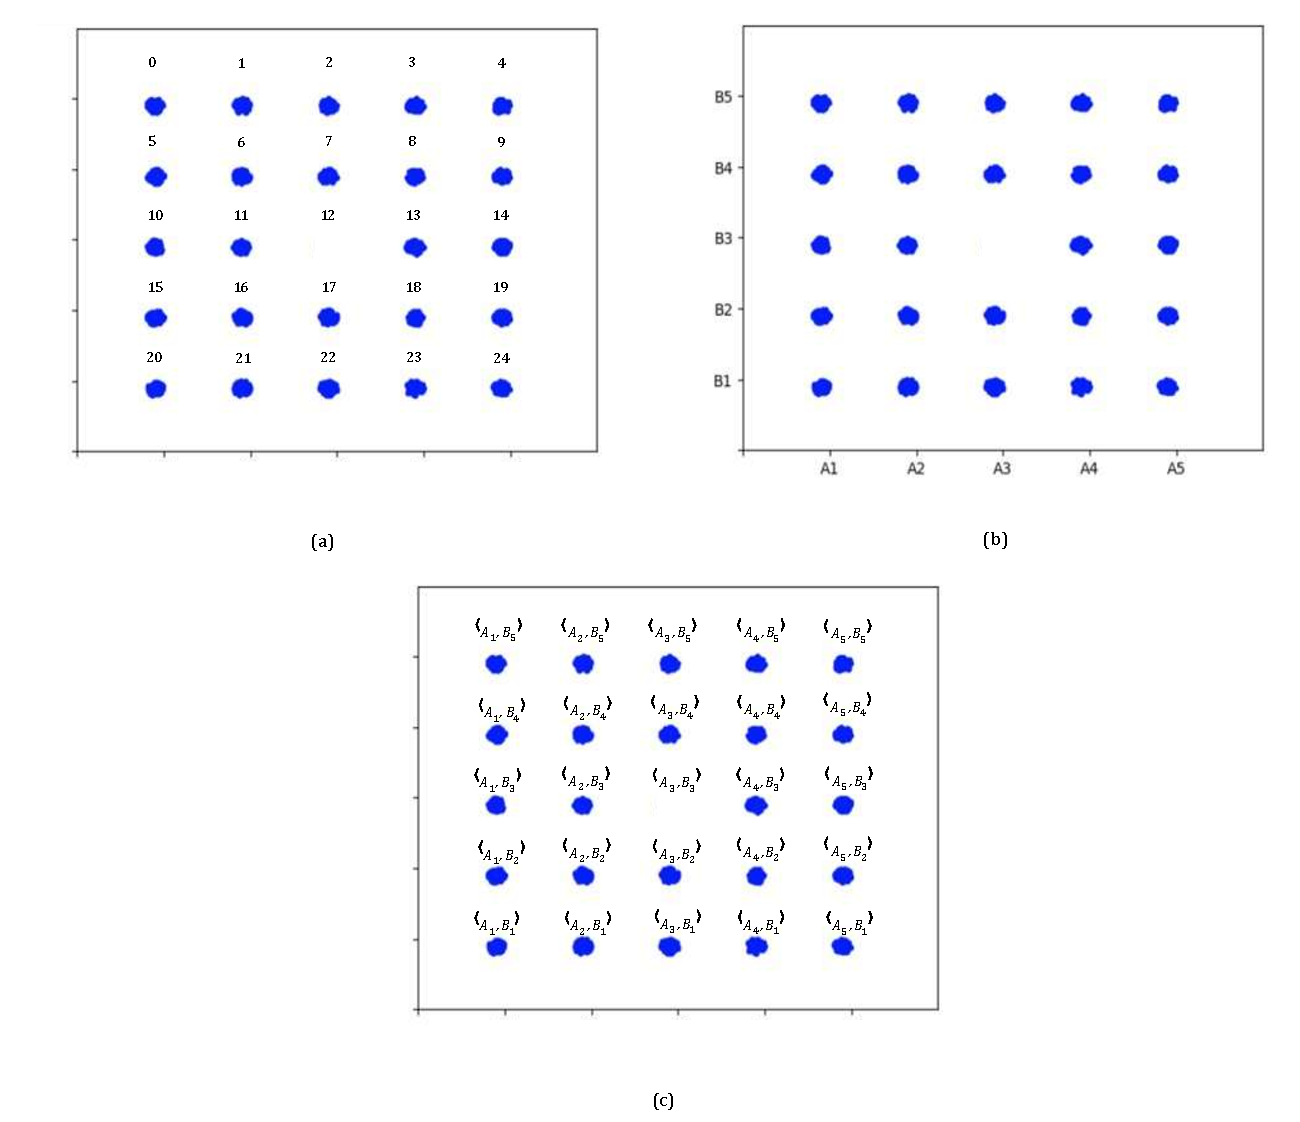
\includegraphics[width=0.8\linewidth]{figures/2dapproach.pdf}
        \caption{Illustration of different approach on 2D point dataset}
        \label{fig:2dapproach}
    \end{figure}
\begin{enumerate}
    \item \textbf{Directly labeling each cluster}: 
    We annotate each cluster, with each cluster corresponding to a label, as shown in figure \ref{fig:2dapproach}.(a). We trained a diffusion model conditioned on class labels $c = {0, 1, 2, ..., 25}$ each label corresponds to a cluster. During the testing phase, we generate each clusters based on the class labels, cluster corresponding to label 12 is not present in the training data. We aim for the generation model to produce it during the testing phase..
    \item \textbf{Compositional visual generation with energy based model }\cite{du2020compositional}:
    We referenced the content of this paper to decompose the problem, approaching image generation from a compositional generation perspective. We annotated each row and column of clusters in the image, as shown in figure \ref{fig:2dapproach}.(b) below, and trained different energy models based on the class labels $c = {A_1, A_2, A_3, A_4, A_5, B_1, B_2, B_3, B_4, B_5}$. In this example, we train ten energy-based models. During the testing phase, we combine any two energy-based models to generate clusters. We aim for the combination of the energy-based models with labels $A_3$ and $B_3$ to generate the missing cluster in the center.
    \item \textbf{Compositional visual generation with composable diffusion models}\cite{liu2022compositional}:
    We referenced the content of this paper to decompose the problem, approaching image generation from a compositional generation perspective. We annotated each row and column of clusters in the image, as shown in figure \ref{fig:2dapproach}.(b) below, and trained different energy models based on the class labels $c = {A_1, A_2, A_3, A_4, A_5, B_1, B_2, B_3, B_4, B_5}$. In this example, we train ten diffusion models. During the testing phase, we combine any two diffusion models to generate clusters. We aim for the combination of the diffusion models with labels $A_3$ and $B_3$ to generate the missing cluster in the center.
    \item \textbf{Compositional generation with compositional class label(ours)}:
    For each cluster in the image, we assigned a corresponding compositional class label composed of two class labels, as shown in figure \ref{fig:2dapproach}.(c). We trained our model conditioned on compositional class labels $c, c = <A_1, B_1>, <A_1, B_2>, ..., <A_5, B_5>$.During the testing phase, we aim for the cluster generated with the condition $<A_3, B_3>$ to appear in the center of the plot.
\end{enumerate}
\subsection{Experiment results}
We use MultiLayer Perceptron(MLP)\cite{taud2018multilayer} in our experiment. Detailed hyperparameters are provided in table \ref{tab:ccdm_mlp}.

\begin{table} [H]
    \centering
    \begin{tabular}{cc} 
         \hline
         & CCDM (MLP as denoising model) \\
         \hline
         Diffusion steps & 50\\
         Noise Schedule & linear \\
         Number of Fully Connected Layer & 3 \\
         Batch Size & 512 \\
         Epochs & 100 \\
         Learning Rate & $2 \times 10^{-4}$ \\
         Embedded Dimension & 128 \\
    \bottomrule[0.5mm]
    \end{tabular}
    \caption{Hyperparameters for CCDM(without attention) trained on the 2D Point Dataset.}
    \label{tab:ccdm_mlp}
\end{table}

\begin{figure} [H]
    \centering
    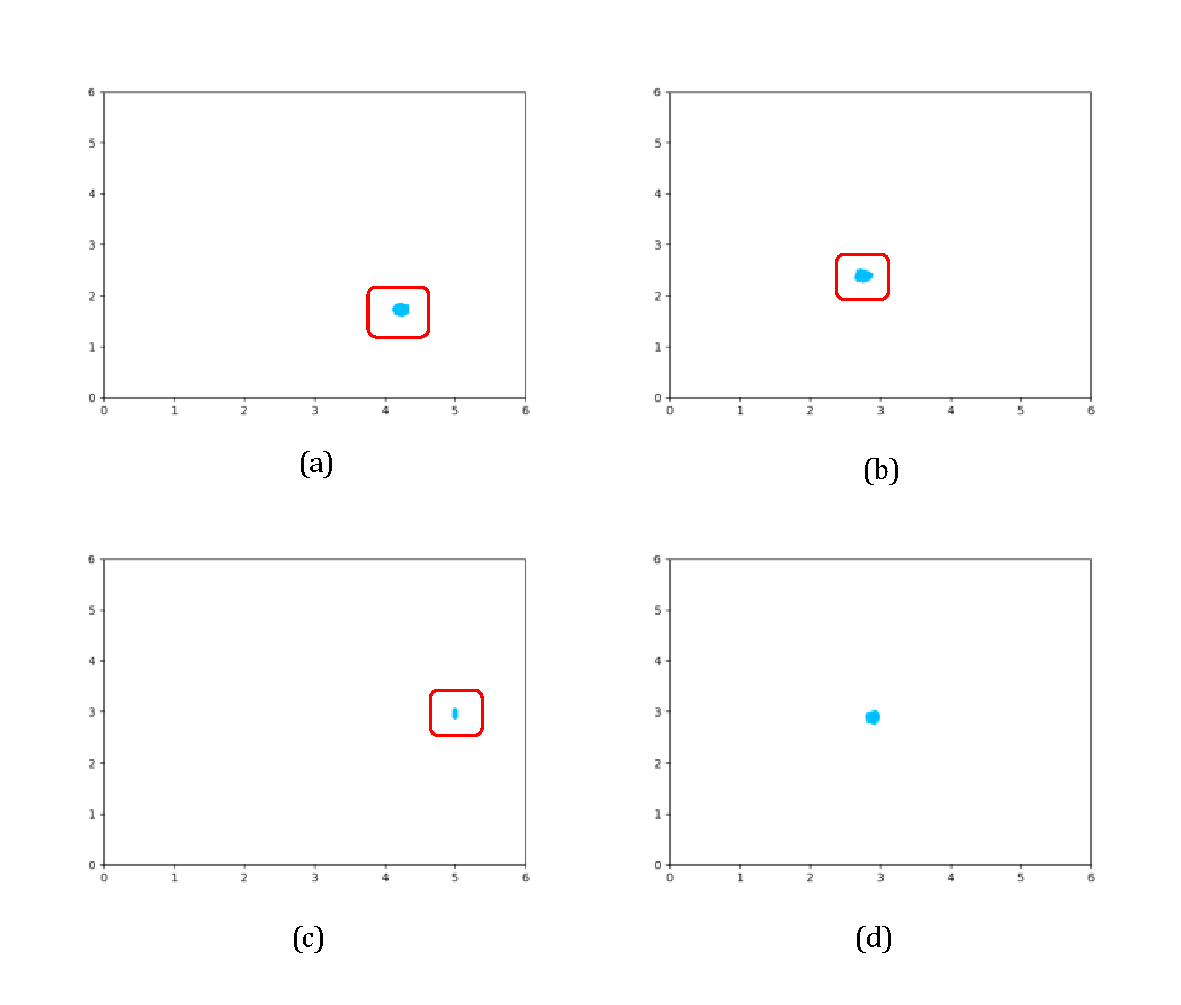
\includegraphics[width=0.8\linewidth]{figures/2dresult.pdf}
    \caption{The unseen clusters generated by the four different methods mentioned above}
    \label{fig:2dresult}
\end{figure}

As shown in figure \ref{fig:2dresult},the unseen cluster generated from first three methods fail were not at the correct position and all shifted during the testing phase. On the contrary, our method can accurately generate the unseen cluster in the center. With this success on this toy dataset, we have gained more confidence in the compositional class label-to-image diffusion model.



\section{Goal}
Let $C_1, C_2, ..., C_m$ be set of category labels for each condition, $|C_1| = N_1, |C_2| = N_2, |C_m| = N_m$. The set of all compositions $U, |U| = N_1 \times N_2 \times \cdots \times N_m, S \subset U$  is the set of available compositions. Our goal is using the available composition $c_i, c_i \in S$ to generate all compositions $c_j, c_j \in U$.

Our research aims to applying compositional cognitive abilities to image generation emphasizes "learning from old compositional concepts and generalizing to new compositional concepts", achieving compositional zero-shot image generation.
\begin{figure} [H]
    \centering
    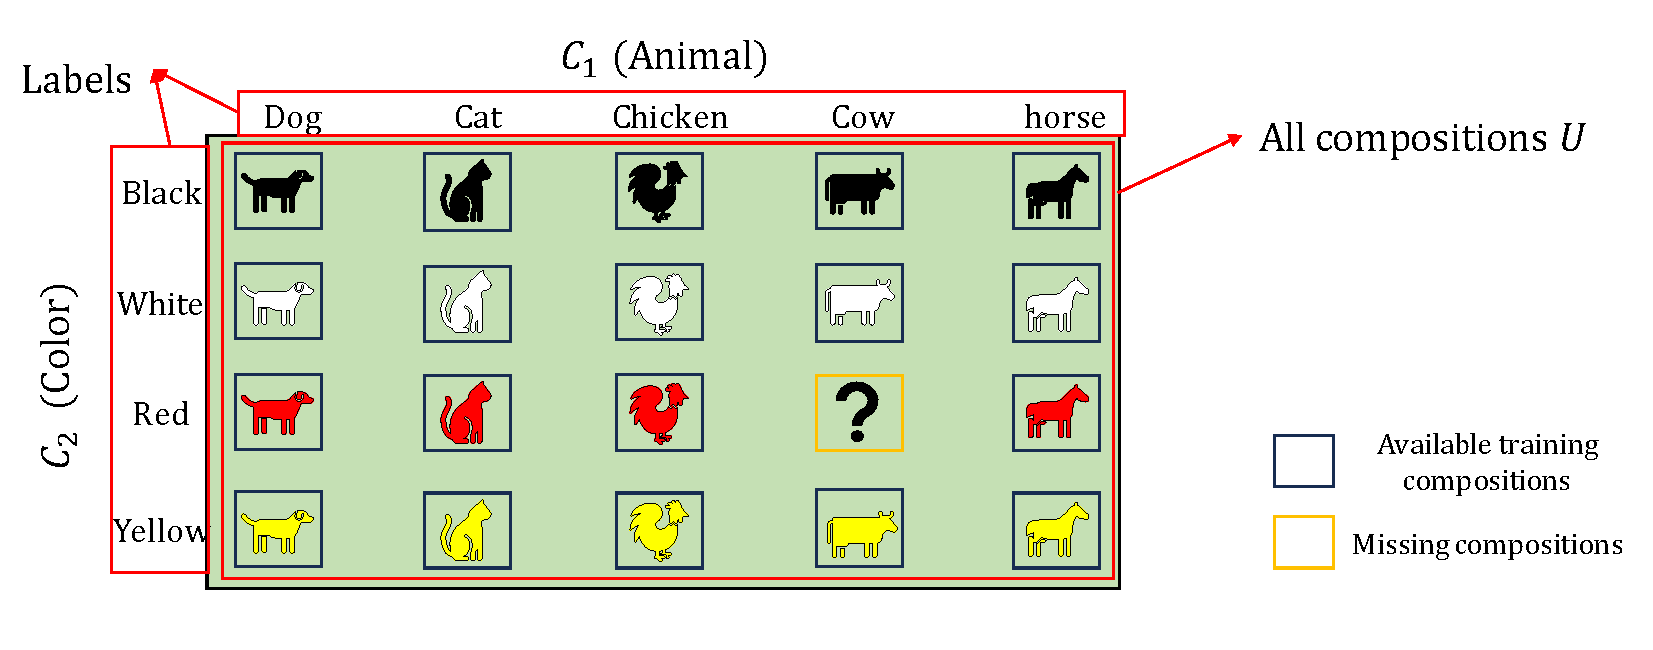
\includegraphics[width=1\linewidth]{figures/goal.pdf}
    \caption{Illustraion of Compositional Zero-shot image generation}
    \label{fig:compositional zero shot}
\end{figure}

As illustrate in figure\ref{fig:compositional zero shot},$C_1$ represents the species of animals, and $C_2$ represents colors. They respectively have the categories "Dog", "Cat", "Chicken", "Cow", "Horse", "Black", "White", "Red", and "Yellow". In total, there can be 20 compositions formed from these categories. However, our training dataset only contains 19 of these compositions. Our goal is to generate all compositions using the limited training compositions.


\section{Contribution}
The contributions of this paper are summarized in the followings:
\begin{itemize}
    \item We propose a novel method for class label-to-Image generation, utilizing various categories of class labels and employing compositional class labels to generate the desired images. This enhances the controllability of the Diffusion model when using class labels as conditions, enabling the generation of more precise images and even producing images that have never been seen in the original dataset.
    \item On the application scenario, our model utilizes multiple categories of class labels to generate images. Compared to models that generate images from text, the process of image generation is simpler and faster. There is no need for meticulous design of inputs to produce the desired images. Additionally, our approach eliminates the necessity for large pretrained language models and the substantial amount of data and data preprocessing typically required for training language models, such as prompt engineering.
    \item Our method offers an efficient way to expand and enrich the original dataset, addressing issues related to data imbalance or absence. Since our model is trained using the original dataset, it effectively addresses the augmentation of the dataset by generating various combinations of data, filling gaps in missing or underrepresented classes. When utilizing compositional class labels as inputs, the generated images exhibit diversity, preventing an overly uniform representation and promoting a more varied dataset. Importantly, this approach avoids the generation of out-of-distribution data. Following the generation of composite images, a classification model is employed to filter the images. This framework serves as an efficient and effective way to expand and enhance the original dataset.
\end{itemize}

The rest of this thesis is organized as follows. Chapter~\ref{chapter:relatedwork} briefly describes related work. Chapter~\ref{chapter:preliminary} describes more details about diffusion models. Chapter~\ref{chapter:method} details the proposed method and architecture. Chapter~\ref{chapter:experiments} shows our experiment results. Chapter~\ref{chapter:conclusion} concludes this thesis.


